\documentclass{article}
\usepackage{v-equation}
\vgeometry
\usepackage{v-electrostatics}
\begin{document}

\def\gdrive{https://drive.google.com/drive/folders/1xF2jyRsVdntXaRQ2FSwrDm8V_AO16PY_?usp=share_link}
\vtitle[Electric field:Dipole]

\begin{center}
\begin{tikzpicture}
[thick, cap=round]
\def\a{1}
	\tzcoor*(-\a, 0)(Q'){$-q$}[b](5pt)
	\tzcoor*(\a, 0)(Q){$+q$}[b](5pt)
	\tzcoor*(45:3)(A){}
	\tzline(Q)(Q')
	\tzline+[->]<0.5, -0.5> (Q)(1, 0){$\vec{p}$}[r]
	\tzline(0, 0)(A){$r$}[ml]
	\tzanglemark(\a, 0)(0, 0)(A){$\theta$}
	\tzline+[->](A)(90:1.5){$\vec{E}$}[ar]
	\tzline+[->](A)(45:1.5){$\vec{E}_r$}[r]
	\tzline+[->](A)(135:1.5){$\vec{E}_\theta$}[al]
\end{tikzpicture}
\end{center}
\vspace*{\fill}
\addtolength{\jot}{3ex}
\begin{align*}
	E_r &= \K \cdot \dfrac{2p}{r^3}\cos\theta\\
	E_\theta &= \K \cdot \dfrac{p}{r^3}\sin\theta\\
	E &= \K \cdot \dfrac{p}{r^3}\sqrt{1+3\cos^2\theta}
\end{align*}
\vspace*{\fill}

\pagebreak

\vspace*{\fill}
\begin{center}
    \fbox{\qrcode[height=2cm]{\gdrive}}
\end{center}
\vspace*{\fill}
\end{document}
